\documentclass[bachelor, och, referat]{SCWorks}
\usepackage[T2A]{fontenc}
\usepackage[utf8]{inputenc}
\usepackage{graphicx}
\usepackage[sort,compress]{cite}
\usepackage{amsmath}
\usepackage{amssymb}
\usepackage{amsthm}
\usepackage{fancyvrb}
\usepackage{longtable}
\usepackage{array}
\usepackage[english,russian]{babel}
\usepackage[colorlinks=true]{hyperref}

\begin{document}

% Кафедра (в родительном падеже)
\chair{дискретной математики и информационных технологий}

% Тема работы
\title{Цветовые гармонии и их применение}

% Курс
\course{2}

% Группа
\group{221}

% Специальность/направление код - наименование
\napravlenie{09.03.01 "--- Информатика и вычислительная техника}

% Фамилия, имя, отчество в родительном падеже
\author{Мусатова Федора Алексеевича}

% Заведующий кафедрой
\chtitle{доцент, к.\,ф.-м.\,н.} % степень, звание
\chname{Л.\,Б.\,Тяпаев}

% Научный руководитель (для реферата преподаватель проверяющий работу)
\satitle{старший преподаватель} %должность, степень, звание
\saname{М.\,В.\,Белоконь}

% Год выполнения отчета
\date{2024}

\maketitle

\tableofcontents

\newpage

\intro
Цветовые гармонии — важный элемент в дизайне, искусстве и маркетинге. Они позволяют создавать визуально привлекательные композиции и задавать настроение. В данном реферате рассмотрены основные цветовые схемы и их применение.

\section{Аналоговая гармония (динамичная и мягкая)}
Аналоговая гармония — это сочетание цветов, расположенных рядом друг с другом на цветовом круге. Примером может служить зелёный, жёлто-зелёный и жёлтый. Эти цвета создают мягкие и спокойные композиции, поскольку их тона близки по своему восприятию. Аналоговая гармония может быть как динамичной, так и мягкой. Динамичные схемы используют более яркие оттенки, создавая ощущение движения, а мягкие схемы используют приглушённые оттенки, чтобы передать спокойствие.
Аналоговая гармония объединяет цвета, которые находятся рядом друг с другом на цветовом круге, создавая схему, которая выглядит гармонично и естественно. Это сочетание напоминает цветовые палитры, которые встречаются в природе, например, закаты и пейзажи. Цвета в аналоговой гармонии мягко переходят друг в друга и придают композиции единство, не вызывая визуального напряжения.
Для усиления эффекта можно использовать насыщенные или пастельные оттенки, добиваясь динамики или умиротворения соответственно. Так, яркие оттенки добавляют энергии и подходят для динамичного дизайна — они создают движение и визуальную активность, идеально подходящие для графического и веб-дизайна, рекламы. Пастельные или мягкие оттенки в аналоговой гармонии создают спокойные и приятные образы, что идеально подходит для интерьера и оформления одежды, где требуется мягкость [2].

Применение. Эта схема часто встречается в природе и отлично подходит для создания естественных и гармоничных композиций, таких как пейзажи или интерьер, где требуется уют и спокойствие.

На рисунке 1 представлен пример аналоговой гармонии динамичной и мягкой.
\begin{figure}
        
\includegraphics[width=0.6\linewidth]{analog_example.png} 
        \caption{Аналоговая гармония (динамичная и мягкая)}
 \end{figure}

\section{Цветовая схема родственноконтрастных цветов}
Родственноконтрастные цвета — это оттенки, которые содержат общий цветовой элемент, но отличаются насыщенностью или светлотой. Например, тёмно-синий и светло-зелёный. Эти цвета не являются аналогами, но имеют гармоничные связи благодаря общим компонентам. Схема создаёт ощущение контраста, но без резких конфликтов между цветами.
Цветовая схема родственноконтрастных цветов отличается тем, что в ней участвуют оттенки, связанные общим компонентом, но расположенные на некотором расстоянии друг от друга на цветовом круге. Благодаря этому контраст создаётся не слишком жёсткий, но при этом сохраняется разнообразие. Например, схема может включать сине-зелёный и оранжево-красный, которые обеспечивают баланс и спокойствие с добавлением контраста, но не выглядят агрессивно, как комплементарные сочетания.
Такие схемы часто применяются в изобразительном искусстве, когда художник хочет создать богатую и сложную композицию с минимальными цветовыми конфликтами. В интерьере эта схема подходит для создания элегантного пространства с умеренной динамикой, где выделяются детали и текстуры, добавляющие глубины и гармонии [4].

Применение. Используется в моде и интерьере для создания интересных цветовых переходов без сильных диссонансов, когда нужно показать разнообразие, но сохранить общую гармонию.

На рисунке 2 представлен пример цветовой схемы родственноконтрастных цветов.
\begin{figure}
        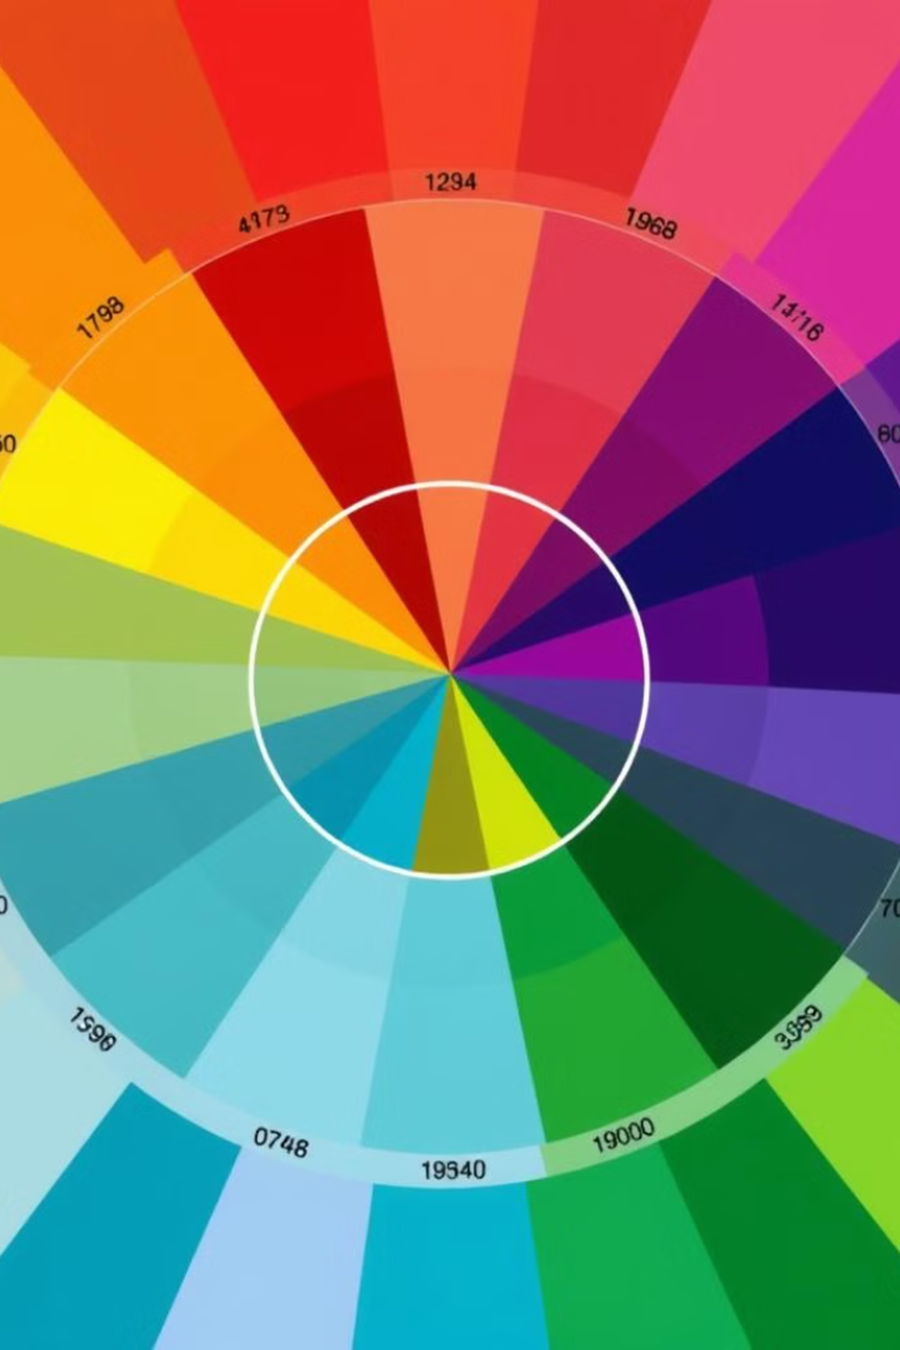
\includegraphics[width=0.6\linewidth]{related_contrast_example.png} 
        \caption{Цветовая схема родственноконтрастных цветов}
 \end{figure}

\section{Цветовая схема контрастных цветов}
Контрастные цвета расположены на противоположных сторонах цветового круга. Это, например, синий и оранжевый. Контраст между ними создаёт сильную динамику и напряжение. Такие цвета привлекают внимание и могут быть использованы для выделения важных элементов.
Контрастные цвета — это цвета, расположенные на противоположных сторонах цветового круга, например, синий и оранжевый или красный и зелёный. Контраст между ними позволяет создать напряжённое и эффектное сочетание, которое сразу привлекает внимание. Эти цвета дополняют друг друга и усиливают восприятие каждого, но их сочетание может быть сложно использовать, не перегружая композицию.
Эта схема широко используется в коммерческом дизайне, особенно в рекламе и маркетинге, где важно быстро завладеть вниманием аудитории. Например, в рекламе яркие контрастные цвета выделяют ключевые элементы и послания, помогая донести информацию до зрителя. В моде контрастные цвета часто применяются для создания смелых и выразительных образов, особенно в случае с аксессуарами и спортивной одеждой [2].

Применение. Реклама, графический дизайн, где важно привлечь внимание зрителя, например, в создании логотипов или постеров.

На рисунке 3 представлен пример цветовой схемы контрастных цветов.
\begin{figure}
        
\includegraphics[width=0.6\linewidth]{contrast_example.png} 
        \caption{Цветовая схема контрастных цветов}
 \end{figure}

\section{Комплементарные цвета}
Комплементарные цвета — это цвета, которые дополняют друг друга, находясь на противоположных сторонах цветового круга. Пример: красный и зелёный. Они усиливают друг друга, создавая яркий контраст и живость. Однако их использование требует осторожности, так как слишком сильное противостояние может вызвать визуальный дискомфорт.
Комплементарные цвета усиливают друг друга и расположены на противоположных концах цветового круга, такие как красный и зелёный, синий и оранжевый. Они привлекают внимание и придают глубину, если используются в сбалансированных пропорциях. Одной из интересных особенностей комплементарных цветов является их способность создавать визуальные эффекты — например, вибрацию, когда они размещены рядом и равны по насыщенности.
В изобразительном искусстве комплементарные цвета применяются для создания иллюзии пространства и объёма. Контраст между ними помогает выделить форму и текстуру. Например, в портретах или натюрмортах, где используются тёплые и холодные комплементарные оттенки, создаётся динамичное и запоминающееся изображение [2].

Применение. Комплементарные цвета часто используются в живописи для создания глубины и контраста, а также в дизайне интерьеров, чтобы выделить определённые объекты.

На рисунке 4 представлен пример комплементарных цветов.
\section{Динамичные и мягкие схемы}
Эти две схемы основаны на восприятии насыщенности и яркости цветов. Динамичные схемы используют насыщенные и яркие цвета, что создаёт энергию и движение в композиции. Мягкие схемы включают пастельные, приглушённые тона, которые дают ощущение умиротворения и гармонии.
\begin{figure}
        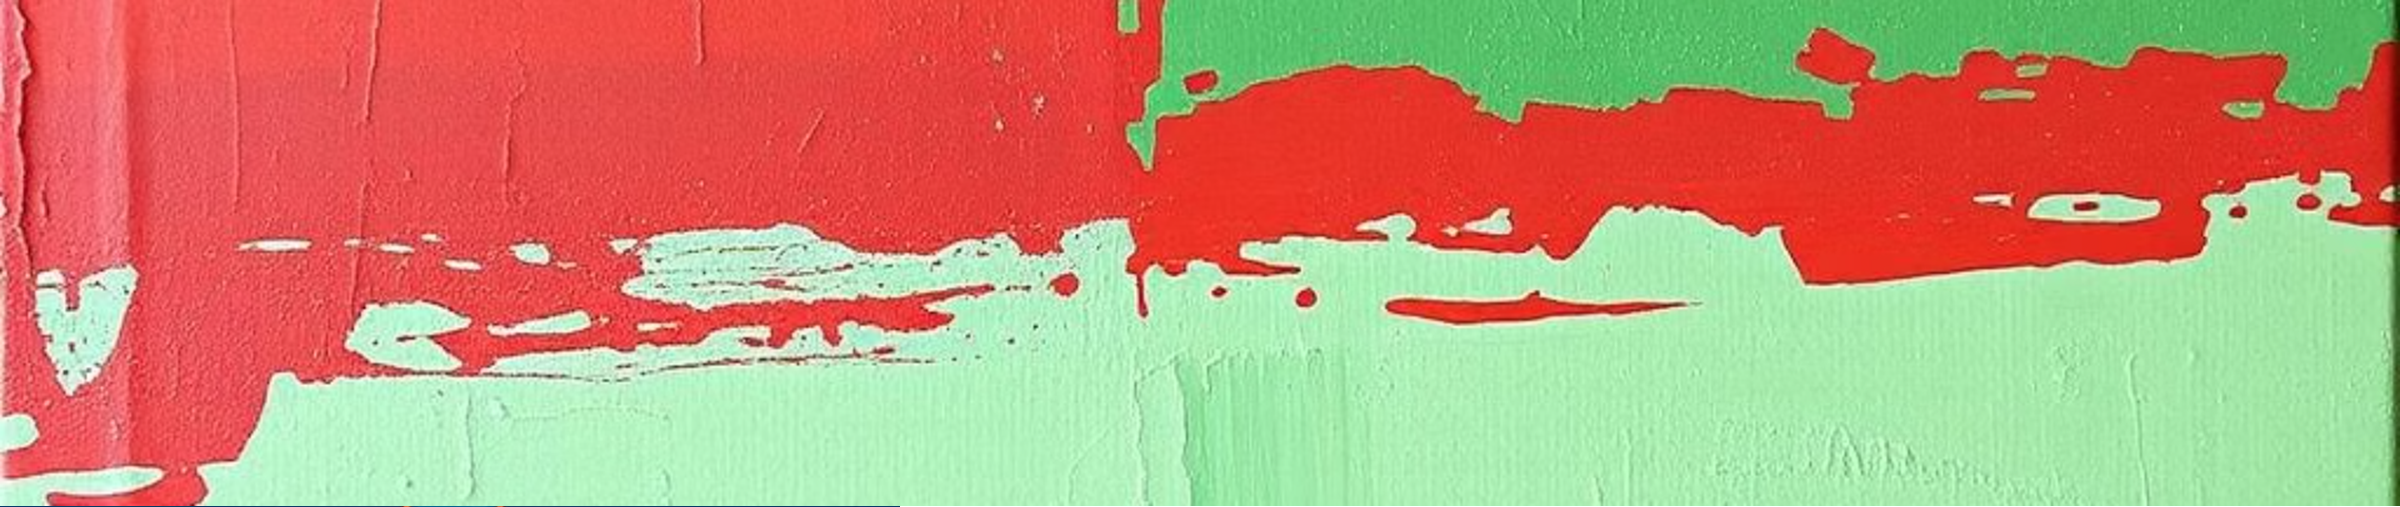
\includegraphics[width=0.6\linewidth]{complementary_example.png} 
        \caption{Комплементарные цвета}
 \end{figure}
Динамичные схемы построены на основе ярких, насыщенных цветов, которые создают впечатление движения и энергии. Они применяются в случаях, когда требуется передать активность, энергию и яркость. Например, спортивные бренды и реклама событий активно используют такие схемы для привлечения аудитории, акцентируя внимание на активном стиле жизни.
Мягкие схемы, наоборот, используют пастельные и светлые оттенки, которые создают умиротворение и гармонию. Такие схемы востребованы в интерьере, где требуется создать атмосферу спокойствия и расслабления. Мягкие цветовые схемы также находят применение в детской одежде и дизайне, так как их нежные оттенки не создают визуального давления и легко воспринимаются [2].

Применение. Динамичные схемы отлично работают в спортивной одежде и рекламных материалах, а мягкие схемы — в интерьерах и ландшафтных дизайнах.

\section{Триадные гармонические схемы}
Триадная схема включает три цвета, равномерно расположенные на цветовом круге. Пример: красный, синий и жёлтый. Эти цвета создают динамическое равновесие и могут использоваться для создания смелых, выразительных композиций. Однако важно сохранять баланс, чтобы не перегрузить композицию.
Триадные схемы строятся из трёх цветов, которые равномерно расположены на цветовом круге. Примером могут быть такие сочетания, как красный, синий и жёлтый или фиолетовый, зелёный и оранжевый. Такая схема предлагает баланс между всеми тремя цветами, что позволяет создавать яркие и гармоничные композиции. При этом каждый цвет вносит свою роль в композицию, не доминируя над другими.
Часто триадные схемы используют в логотипах и брендировании, где нужно передать разнообразие и оригинальность. Эта схема также востребована в графическом дизайне и искусстве, где она помогает создавать яркие и выразительные композиции без излишней резкости.

Применение. Часто используется в логотипах, когда нужно передать разнообразие и активность, как в случае с логотипами крупных компаний.

\section{Сплит-комплементарная гармония}
Сплит-комплементарная схема включает один основной цвет и два цвета, находящихся рядом с его комплементарным цветом на цветовом круге. Это создаёт контраст, но менее жёсткий, чем при использовании комплементарной схемы. Пример: синий, жёлто-оранжевый и красно-оранжевый.
Сплит-комплементарная схема основана на выборе одного основного цвета и двух дополнительных цветов, которые расположены рядом с комплементарным цветом. Например, если выбрать синий, то дополнительными цветами могут быть жёлто-оранжевый и красно-оранжевый. Это сочетание создаёт умеренный контраст и обеспечивает баланс между яркостью и гармонией.
Сплит-комплементарные схемы дают больше гибкости по сравнению с традиционными комплементарными сочетаниями, так как позволяют избегать слишком резкого визуального напряжения. Это популярный выбор для моды, декора и графического дизайна, когда требуется лёгкость и контраст без излишнего давления [2].

Применение. Эта схема помогает создавать контрастные, но более сбалансированные композиции. Её часто применяют в моде и дизайне интерьеров.

\section{Тетрадная гармоническая схема}
Тетрадная схема использует четыре цвета, состоящие из двух пар комплементарных цветов. Это сложная, но интересная схема, которая позволяет создать богатую и многослойную палитру. Пример: синий, оранжевый, зелёный и красный.
Тетрадная схема включает четыре цвета, образованных из двух пар комплементарных оттенков, таких как синий, оранжевый, красный и зелёный. Эта схема создаёт богатое сочетание, которое выглядит разнообразно, но требует осторожности в использовании, чтобы не перегрузить композицию. Тетрадные схемы хорошо подходят для создания сложных, многослойных образов.
Часто применяются в дизайне интерьеров и моде, где важно привнести разнообразие, сохраняя при этом гармонию. Тетрадные схемы также используются в графике и иллюстрации, где важен баланс между яркостью и сложностью [2].

Применение. Используется в сложных дизайнах, где требуется многообразие, но при этом важно сохранить общую гармонию.

\section{Попарно-комплементарная схема}
Попарно-комплементарная схема состоит из двух комплементарных пар цветов. Эта схема создаёт мощный контраст, но из-за большого количества цветов её сложнее контролировать. Пример: фиолетовый, жёлтый, синий и оранжевый.
Попарно-комплементарная схема также включает две пары комплементарных цветов, таких как фиолетовый с жёлтым и синий с оранжевым. Такое сочетание создаёт мощный визуальный эффект и придаёт композиции глубину и контраст. Использование четырёх цветов, подобранных таким образом, требует контроля над насыщенностью и распределением, чтобы избежать перегрузки.
Попарно-комплементарная схема популярна в современной моде и рекламе, где требуется привлечь внимание к отдельным элементам. В искусстве эта схема позволяет создавать яркие и запоминающиеся образы, сохраняя баланс и комплексность [8].

Применение. Эта схема подходит для создания экспрессивных и живописных композиций, особенно в искусстве и рекламе.

\section{Аналого-комплементарная схема}
Аналого-комплементарная схема включает основной цвет, два аналоговых к нему цвета и один комплементарный цвет. Пример: зелёный, сине-зелёный, жёлто-зелёный и красный. Это сочетание позволяет достичь баланса между гармонией аналогов и контрастом комплементарного цвета.
Аналого-комплементарная схема сочетает основной цвет с двумя аналоговыми оттенками и одним комплементарным цветом. Например, для зелёного это могут быть сине-зелёный, жёлто-зелёный и красный. Это придаёт композиции баланс между спокойствием и контрастом, создавая эффектные и в то же время гармоничные образы.
Эта схема используется в веб-дизайне, моде и маркетинге, где требуется сохранить гармонию и привлечь внимание к ключевым элементам [5].

Применение. Эта схема часто используется в веб-дизайне и маркетинге для создания акцентов в гармоничных композициях.

\conclusion
Цветовые гармонии играют ключевую роль в создании визуально привлекательных композиций. Каждая схема имеет свои особенности и подходит для различных целей — от интерьеров до рекламы. Грамотное использование этих схем позволяет создавать эстетически приятные и функциональные решения.

%Список литературы
\newpage
\section*{Список использованных источников}
\begin{enumerate}
    \item Альберс Й. Interaction of Color. Yale University Press, 1971.
    \item Тернбулл Д. Color: A Natural History of the Palette. Random House, 2004.
    \item Альберс Й. The Art of Color. Yale University Press, 1975.
    \item Гурни Дж. Color and Light: A Guide for the Realist Painter. Andrews McMeel Publishing, 2010.
    \item Adobe. Adobe Color Wheel [Электронный ресурс]. URL: \url{https://color.adobe.com} (дата обращения: 15.10.2024).
    \item Зальцман Дж. The Psychology of Color in Marketing and Branding [Электронный ресурс]. URL: \url{https://www.colorpsychology.org} (дата обращения: 15.10.2024).
    \item Smashing Magazine. Color Theory for Designers [Электронный ресурс]. URL: \url{https://www.smashingmagazine.com} (дата обращения: 15.10.2024).
    \item CreativeBloq. Color Theory: A Guide to Color in Art and Design [Электронный ресурс]. URL: \url{https://www.creativebloq.com} (дата обращения: 15.10.2024).
\end{enumerate}

\end{document}
